%-------------------------------------------------------------------------------
\section{Gradient Analysis Framework}
%-------------------------------------------------------------------------------

The gradient analysis framework works similarly to autodifferentiation, computing the gradient of each operation and using the results as inputs to the next gradient. However, unlike autodifferentiation, nonsmooth functions are handled by Proximal Gradients, so that a meaningful gradient can be computed over all program operations. Since Proximal Gradients require local Lipschitz Constants to bound their sampling in some cases, Lipschitz Constants are also propogated over the program along with the gradient.

\noindent \textbf{Gradient Propogation with Chain Rule.} We model a program as an arbitrary function $P$, that operates on the system state $x$ and produces a modified system state $x'$. Since programs are generally nonsmooth, we can use subgradients to approximate the gradient of $P$. Programs in general are too complex to model, but since the program $P$ is composed of individual operations whose behavior is known, we model $P$ as a composition of $N$ individual functions on the system state that represent each operation in the program:

\vspace{-10pt}\begin{align*}
P(x) = P_N \circ P_{N-1} \circ \cdots \circ P_2 \circ P_1 (x)
\end{align*}

Subgradients compose under the chain rule, so we apply the same approach used in Automatic Differentation to evaluate the subgradient of $P$,  $\nabla_{sub} P(x)$ by computing the product of the subgradients of each operation in $P$ ~\cite{rockafellar2009variational}. 

\vspace{-10pt}\begin{align*}
  \nabla_{sub} P(x) = \nabla_{sub} P_N * \nabla_{sub} P_{N-1} * \cdots * \nabla_{sub} P_2 * \nabla_{sub} P_1
\end{align*}

This is the same approach used in Automatic Differentiation, but applied to discrete functions and subgradients instead of continuous functions with gradients. Then, instead of attempting to evaluate a subgradient over the program function $P$, which has unknown behavior and operate on a large number of variables, subgradients can be evaluated on the individual operations $P_i$, which have known behavior and usually only operate on 1 or 2 variables.

For some operations that are analytically differentiable on continuous variables, the subgradient of the operation on discrete variables can also be computed analytically. However, the subgradients of nonsmooth operations must be approximated with Proximal Gradients. 

\noindent \textbf{Sampling Bounds with Lipschitz Constants.} In order to bound the samples required to evaluate the Proximal Gradient, Lipschitz Bounds must also be known for each operation. Fortunately, Lipschitz Bounds can be computed for each type of nonsmooth operation in a program based on its behavior and the Lipschitz bounds of its input. This means that in addition to propogating the gradient through a program, we also compute the Lipschitz Constant on each operation based on the Lipschitz Constants of its inputs, and propogate the result to the next function.

In some cases the Lipschitz Constant $K_f$ cannot be derived from knowledge of the function, so it is estimated by sampling the function at $x \pm K$ and taking the maximum difference.

\noindent \textbf{Partial Derivatives.} A gradient is composed of partial derivatives with regard to each part of the input, so when defining rules for computing the gradient we focus on partial derivatives with regard to the variable in the system state that was first marked for tracking, which is denoted $x_i$. Typically $x_i$ is a byte in an input read from a file or socket, but may also be an internal program variable.


\noindent \textbf{Program Inputs.} In the case where $g$ and $h$ are direct inputs to the program, such as bytes read from a file, we consider them to be identity functions with a partial derivative of 1 if they operate on the byte of the input that the partial derivative is being taken with regard to, and 0 otherwise. The Lipschitz Constant in this case is also 1.

\noindent \textbf{Propogation rules.} We then define gradient and Lipschitz Constant propogation rules as follows, where $f$ represents the current operation and $g$ and $h$ represent the prior operations on its input.

\begin{enumerate}
  \item \textbf{Addition and Multiplication.} Addition and multiplication, as well as subtraction, are examples of discrete functions whose subgradients can still be computed analytically and therefore do not require sampling. The partial derivatives and associated Lipschitz Constants with regard to the $i$th input variable $x_i$ can then be computed as follows based on the definition of $f$ as $f\left(g, h\right) = g+h$:

\vspace{-10pt}\begin{align*}
  K_f &= K_{g} + K_{h} &\tfrac{df}{dx_i} &= \tfrac{dg}{dx_i} + \tfrac{dh}{dx_i}
\end{align*}

Multiplication can likewise rely on analytical derivatives as it is a linear operation:

\vspace{-10pt}\begin{align*}
  K_f &= h*K_{g} + g*K_{h} & \frac{df}{dx_i} &= h\frac{dg}{dx_i} + g\frac{dh}{dx_i}
\end{align*}

    \gabe{These are pretty obvious, textual description may be sufficient.}


\item \textbf{Integer Division.} Unlike division with continuous values, division on integers is not a linear function because any fractional portion of the result is truncated. Therefore sampling the function is necessary to evaluate an accurate partial derivative. To compute the Lipschitz Constant, we use the quotient rule and consider the case that causes the maximum possible change in $f$, where $\tfrac{dg}{dx_i} = K_g$, and $\tfrac{dh}{dx_i} = -K_h$.

\vspace{-10pt}\begin{align*}
  K_f &= \frac{K_g h + K_h g}{h^2} & 
  \frac{df}{dxi} &= prox_{\nabla f}\left(\bar{x}, K_f, \lambda\right)
\end{align*}

\item \textbf{Modulo Operations.} Like integer division, modulo operations are also generally nonsmooth and require evaluating the proximal gradient. In cases the modulo operand is constant, which we found usually the case in our test programs, the Lipschitz Constant for the modulo function is simply the modulo operand:

\vspace{-10pt}\begin{align*}
  K_f &= h &
  \frac{df}{dxi} = prox_{\nabla f}\left(\bar{x}, K_f, \lambda\right)
\end{align*}

In cases where the derivative of the modulo operand is nonzero, the Lipschitz Constant is estimated by sampling and used to evaluate the Proximal Gradient. 


\item \textbf{Shift Operations.} Shift operations can be defined as a multiplication with an exponent, but have the additional condition that bits shifted past the width of the datatype are dropped. Therefore the Lipschitz Constant is also estimated by sampling and used to evaluate the Proximal Gradient.


  \gabe{May want to combine integer division, modulo and shift.}

\item \textbf{Bitwise Operations.} When one of the operands of a bitwise operation is a constant, or at least has a 0 derivative with regard the marked input, the Lipschitz Constant can be set the value of the highest set bit in the constant operand. However, in cases where both operands have nonzero derivatives, the Lipschitz Constant must be estimated and used to evaluate the Proximal Gradient. 


\item \textbf{Memory Indexing.} Indexing into an array in memory can be modeled as an arbitrary nonsmooth function $f\left(g\right)$. Since we cannot derive the Lipschitz Constant $K_f$ from knowledge of the function, we estimate it by sampling the function at $g \pm g'$ and taking the maximum difference. The proximal gradient can be computed using the estimated Lipschitz Constant

%\begin{align*}
  %f\left(g\right) &= \textrm{mem}\left[g\right]\\
  %\frac{df}{dxi} &= prox_{\nabla f}\left(\bar{x}, K_f, \lambda\right)
%\end{align*}

\item \textbf{Load Operations.} Load operations will normally take on the saved partial derivative of whatever variable was originally saved to that memory location. However, there is possibility that one or more types with smaller bit widths are being loaded into a single larger width type. In these cases each partial derivative and Lipschitz Constant associated with an address being loaded, if there are more than one, is shifted by its offset with the base address and summed with the others.

\vspace{-10pt}\begin{align*}
  K_f &= \sum_j K_j 2^{offset_j} &
  \frac{df}{dxi} &= \sum_j \frac{d \textrm{addr}_j}{dx_i}2^{offset_j}
\end{align*}


\item \textbf{Integer Branches.} In cases where a variable can take on different values based on which portion of the branch was executed, we model the branch and subsequent merge as either a piecewise point function or a piecewise step function, depending on if the branch comparison defines a single value or set of values, such as greater than. In order to the Proximal Gradient on this function, the alternate branch path must be sampled to determine its value in the merge operation. In practice any execution of an alternate path will be invalid, but for many branches will still result in an accurate representation of program behavior. In cases where the sample execution does not return to the merge operator, the alternate branch portion of the piecewise function is considered to be undefined, resulting in a partial deriviative of 0. Once the path has been sampled, the Proximal Gradient can be evaluated on it normally, and the associated Lipschitz Constant can be set to the size of the step in the piecewise function.

  This approach will handle most single branches, but breaks down in the case where multiple nested branches on different values must be bypassed for the merge variable to be set. To handle these cases, when sampling alternate branch paths any subsequent branch encountered can also be sampled, and the Proximal Gradient computed over each branch individually. Figure \ref{fig:branch_exs} shows how this process works on nested branches with two conditions, \tc{x>1} and \tc{set>0}. When the branch is initially executed with \tc{x=0} and \tc{set=0}, the result is \tc{y=0}. To evaluate Proximal Gradient, the first branch is sampled by executing the alternate path with \tc{x=2}. This execution also results in \tc{y=0}, but during it the second nested branch on \tc{set} is encountered and sampled with \tc{set=1}, which results in \tc{y=1}. These samples are then used to form a function that is 1 for \tc{x>1} and \tc{set>0} and 0 elsewhere. The closest point to \tc{x=0, set=0} that gives the greatest change on this function is \tc{x=2, set=1}, so the Proximal Gradient evaluates on that point, resulting in partial derivatives of $\tfrac{dy}{dx}=\tfrac{1}{2}$ and $\tfrac{dy}{dset} = 1$.

\begin{figure}
  %\centering
  \begin{subfigure}{0.38\columnwidth}
    %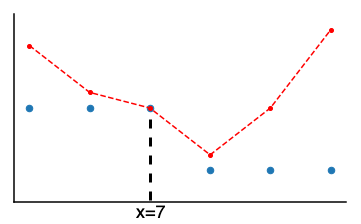
\includegraphics[width=\linewidth]{figs/sosp-working_ex3}
    \begin{lstlisting}
// int x=0 
// bool set=0
int y=0;
if (x>1)
    if (set==1)
        y=1;
    \end{lstlisting}
    %\caption{\label{fig:branch_ex1}Example of nested branch with $\tfrac{dy}{dx}=\tfrac{1}{2}$ and $\tfrac{dy}{dset} = 1$}
  \end{subfigure}
  \hspace{0.1cm}
  \begin{subfigure}{0.58\columnwidth}
    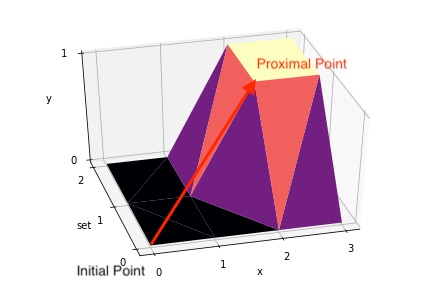
\includegraphics[width=\textwidth]{figs/nested_branch_plot.jpg}
    %\caption{\label{fig:branch_ex2}Surface}
  \end{subfigure}
  \vspace{-0pt}
  \caption{\label{fig:branch_exs}Example of nested branch with $\tfrac{dy}{dx}=\tfrac{1}{2}$ and $\tfrac{dy}{dset} = 1$.}
  \vspace{-0pt}
\end{figure}


\item \textbf{Floating Point Branches.} Unlike derivatives of integer operations, derivatives of floating point operations can generally be computed analytically, as is done in existing autodifferentiation frameworks. The exception to this is branches, which are normally not handled. Like integer branches, we model branches with floating point values as a piecewise step function, and execute the alternate branch path to determine the value of the step. However, unlike integer branches, floating point branches are not locally lipschitz, because they have an infinite slope at the point of discontinuity \gabe{add a figure showing this}, so a Proximal Gradient cannot be evaluated on them. Instead, we apply a Gaussian smoothing function, where the variance of the gaussian used is set according the magnitude of the input derivative.
\end{enumerate}


